\documentclass[11pt, letterpaper]{article}

% --- Packages ---
\usepackage[margin=1in]{geometry}
\usepackage{fontspec}
\usepackage{titlesec}
\usepackage{titletoc}
\usepackage{hyperref}
\usepackage{xcolor}
\usepackage{enumitem}
\usepackage{booktabs}
\usepackage{tabularx}
\usepackage{longtable}
\usepackage{amsmath, amssymb}
\usepackage{tikz}
\usetikzlibrary{arrows.meta, positioning, calc, shapes.geometric, fit, backgrounds}
\usepackage{fancyhdr}
\usepackage{graphicx}
\usepackage{listings}

% --- Colors ---
\definecolor{rimblue}{HTML}{2D5F8A}
\definecolor{rimdark}{HTML}{1A3A54}
\definecolor{rimlight}{HTML}{E8F0F7}
\definecolor{dripcolor}{HTML}{3A7CA5}
\definecolor{jetcolor}{HTML}{D4A03C}
\definecolor{fittingcolor}{HTML}{7B4B94}
\definecolor{rolecolor}{HTML}{4A9E6F}
\definecolor{codebg}{HTML}{F5F5F5}

% --- Fonts ---
\setmainfont{Helvetica Neue}[
  BoldFont = Helvetica Neue Bold,
  ItalicFont = Helvetica Neue Italic,
]
\setmonofont{Menlo}

% --- Hyperlinks ---
\hypersetup{
  colorlinks=true,
  linkcolor=rimblue,
  urlcolor=rimblue,
  citecolor=rimblue,
  pdftitle={Rim Self-Data Protocol: Self-Data Flows},
  pdfauthor={Soradyne Project},
}

% --- Section Formatting ---
\titleformat{\section}
  {\Large\bfseries\color{rimdark}}
  {\thesection}{1em}{}
\titleformat{\subsection}
  {\large\bfseries\color{rimblue}}
  {\thesubsection}{1em}{}
\titleformat{\subsubsection}
  {\normalsize\bfseries\color{rimblue!80}}
  {\thesubsubsection}{1em}{}

% --- Header/Footer ---
\pagestyle{fancy}
\fancyhf{}
\fancyhead[L]{\small\color{gray}Rim Self-Data Protocol}
\fancyhead[R]{\small\color{gray}DRAFT --- \today}
\fancyfoot[C]{\small\thepage}
\renewcommand{\headrulewidth}{0.4pt}

% --- Styled environments (simple, no extra packages) ---
\newenvironment{pseudocode}[1][]
  {\par\medskip\begin{quote}\small
   \ifx&#1&\else\noindent{\bfseries\color{rimblue} #1}\par\smallskip\fi
   \ttfamily}
  {\end{quote}\medskip}

\newenvironment{definition}[1][]
  {\par\medskip\begin{quote}
   \color{rimdark}\rule{\dimexpr\linewidth}{1.5pt}\par\smallskip
   \ifx&#1&\else\noindent{\bfseries #1}\par\smallskip\fi}
  {\par\smallskip\color{rimdark}\rule{\dimexpr\linewidth}{1.5pt}
   \end{quote}\medskip}

\newenvironment{designnote}[1][]
  {\par\medskip\begin{quote}\small
   \ifx&#1&\else\noindent{\bfseries\color{jetcolor} #1}\par\smallskip\fi}
  {\end{quote}\medskip}

% --- Document ---
\begin{document}

% ============================================================
% TITLE PAGE
% ============================================================
\begin{titlepage}
\centering
\vspace*{2cm}

{\Huge\bfseries\color{rimdark} Rim Self-Data Protocol}\\[0.5cm]
{\LARGE\color{rimblue} Self-Data Flows}\\[0.3cm]
{\large Architecture, Concepts, and Design}\\[2cm]

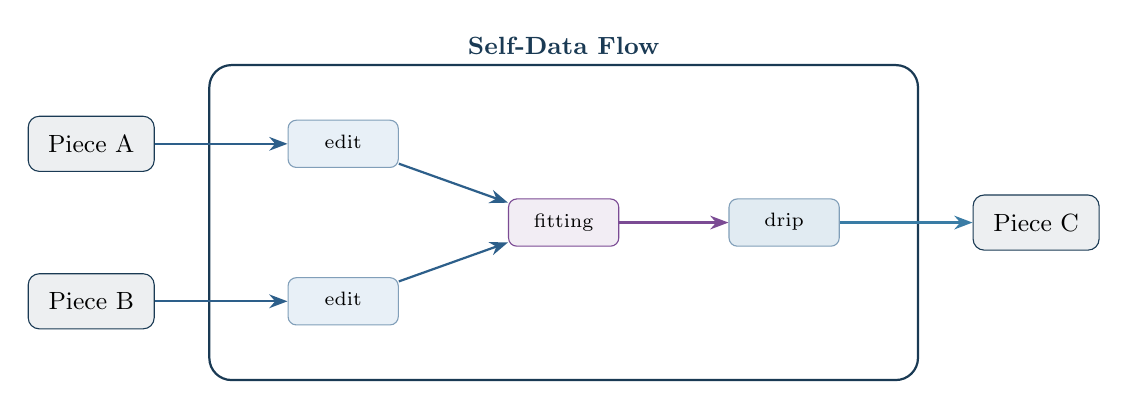
\begin{tikzpicture}[
  stream/.style={draw=rimblue, thick, ->, >=Stealth},
  drip/.style={draw=dripcolor, thick, ->, >=Stealth, densely dashed},
  jet/.style={draw=jetcolor, thick, ->, >=Stealth},
  optional/.style={draw=rimblue, thick, ->, >=Stealth, densely dotted},
  piece/.style={draw=rimdark, fill=rimdark!8, rounded corners=4pt,
                minimum width=1.6cm, minimum height=0.7cm, font=\small},
  streambox/.style={draw=rimblue!60, fill=rimlight, rounded corners=3pt,
                    minimum width=1.4cm, minimum height=0.6cm, font=\scriptsize},
  fitting/.style={draw=fittingcolor, fill=fittingcolor!10, rounded corners=3pt,
                  minimum width=1.4cm, minimum height=0.6cm, font=\scriptsize},
  role/.style={draw=rolecolor, fill=rolecolor!10, rounded corners=3pt,
               minimum width=1.4cm, minimum height=0.6cm, font=\scriptsize},
  flowbox/.style={draw=rimdark, fill=white, rounded corners=8pt, thick, inner sep=10pt},
]
  % Flow boundary
  \node[flowbox, minimum width=9cm, minimum height=4cm] (flow) {};
  \node[above=0pt of flow.north, font=\small\bfseries\color{rimdark}] {Self-Data Flow};

  % Pieces (devices) outside the flow on the left
  \node[piece] (pieceA) at (-6, 1) {Piece A};
  \node[piece] (pieceB) at (-6, -1) {Piece B};

  % Edit streams
  \node[streambox] (editA) at (-2.8, 1) {\strut edit};
  \node[streambox] (editB) at (-2.8, -1) {\strut edit};

  % Fitting (CRDT merge)
  \node[fitting] (fit) at (0, 0) {fitting};

  % Drip (convergent state)
  \node[streambox, fill=dripcolor!15] (drip) at (2.8, 0) {\strut drip};

  % Piece (device) outside the flow on the right
  \node[piece] (pieceC) at (6, 0) {Piece C};

  % Source -> edit stream
  \draw[stream] (pieceA) -- (editA);
  \draw[stream] (pieceB) -- (editB);

  % Edit streams -> fitting -> drip (the convergent path)
  \draw[stream] (editA) -- (fit);
  \draw[stream] (editB) -- (fit);
  \draw[stream, color=fittingcolor] (fit) -- (drip);

  % Drip -> consuming piece
  \draw[stream, color=dripcolor] (drip) -- (pieceC);
\end{tikzpicture}

\vfill

{\large Soradyne Project}\\[0.3cm]
{\color{gray} Draft --- \today}\\[0.3cm]
{\small Reference implementation: \texttt{soradyne\_core} (Rust)}

\end{titlepage}

% ============================================================
% TABLE OF CONTENTS
% ============================================================
\tableofcontents
\newpage

% ============================================================
% PART I: FOUNDATIONS
% ============================================================
\section{Introduction}
\label{sec:intro}

\subsection{What is Self-Data?}

Self-data is data that belongs to a person and exists on their devices. It is not hosted
by a third party on their behalf; it lives where they put it. The Rim Self-Data Protocol
defines how self-data moves between devices, how conflicts are resolved when multiple
devices edit the same data, and how the data is stored, secured, and retrieved.

The protocol assumes maximum heterogeneity among participating devices. A single session
might involve a phone, a laptop, a VR headset, an ESP32 microcontroller, and a robot arm
driven by Python on a Raspberry Pi---each a \emph{piece} in the protocol's terminology
(\S\ref{sec:topology}). Each piece may run different operating systems,
communicate over different transports (Bluetooth Low Energy, TCP, bespoke hardware
interfaces), and have vastly different storage and compute capabilities. The protocol
defines agreements about \emph{what} must happen, and leaves \emph{how} to the
implementations on each device.

\subsection{Design Philosophy}

\begin{itemize}[leftmargin=2em]
  \item \textbf{User-owned}: Data lives on devices the user controls. Third-party
    servers may participate as roles in a flow, but are never the sole authority.
  \item \textbf{Peer-to-peer}: No distinguished leader. Any device can make edits
    offline; all devices converge when they communicate.
  \item \textbf{Device-heterogeneous}: The protocol does not assume homogeneous
    platforms. Implementations exist per-language, per-platform, and conform to
    versioned design documents rather than to a single reference binary.
  \item \textbf{Local-first}: Operations succeed locally and synchronize later.
    Network partitions degrade gracefully; they never block local work.
  \item \textbf{Application-defined}: The protocol provides infrastructure. Applications
    define what their data looks like, how conflicts resolve, and what trade-offs they
    accept. The protocol does not make these decisions for them.
  \item \textbf{Body-proximate, BLE-first}: The protocol treats Bluetooth Low Energy as
    the prototypical network implementation, not TCP/IP. This is a deliberate inversion
    of the usual assumption that sockets or HTTP are basic while wireless variations are
    exotic. The goal is to be as locality-, body-, fashion-, and hardware-centered as
    possible. IP-based transports (TCP, UDP, WebSockets) are available as extensions, but
    the baseline design targets the constraints and affordances of BLE: short range,
    low bandwidth, broadcast-capable, battery-efficient, and physically proximate.
\end{itemize}

\subsection{Scope of This Document}

This document defines \textbf{Self-Data Flows}: the core abstraction by which data is
created, moved, transformed, stored, and queried across devices in the Rim protocol.

It covers:
\begin{itemize}[leftmargin=2em]
  \item The conceptual model: flows, streams, flow roles, fittings, policies
  \item Data geometry: how the spatial, temporal, and structural character of data
    is described so that flows can operate on it uniformly
  \item Worked examples across diverse data types: images, video, sound, spatial
    measurements, photo albums, structured records, and task graphs
  \item The implementer's perspective: how to define new flow types, how versioning
    works, how to extend the system
  \item Security and memorization: policies for data at rest, dissolution, robustness
  \item Device topology: how devices are grouped (capsules), tracked in real time
    (ensembles), and integrated at the hardware level (parures)
\end{itemize}

\subsection{Relationship to Existing Code}

The reference implementation in \texttt{soradyne\_core} (Rust) includes early versions of
many concepts described here. Where the code and this document diverge, the document
represents the intended design. Specifically:

\begin{itemize}[leftmargin=2em]
  \item \texttt{DataChannel<T>} (formerly \texttt{SelfDataFlow<T>}) is a concrete
    implementation of a stream, not a flow.
  \item \texttt{ConvergentDocument<S>} is a tool for implementing a drip stream's
    backing store, not the drip itself.
  \item The \texttt{Flow} trait, \texttt{FlowRegistry}, and \texttt{FlowConfigStorage}
    in \texttt{flow\_core.rs} reflect the bootstrap-from-UUID model described here and
    are directionally correct.
\end{itemize}

% ============================================================
\newpage
\section{Self-Data Flows}
\label{sec:flows}

\begin{definition}[Self-Data Flow]
A self-data flow is a persistent, typed, UUID-identified, authenticated instance of a
bundle of streams, created from a schema for building streams, along with a collection
of policies for how serialized data is moved and transformed between streams, policies
for delegating who performs transmissions and transformations, and policies for exceptions.

New streams may be created according to the schema after the bundle is created.
\end{definition}

\subsection{Identity: The UUID}

Every flow instance has a UUID. This is the stable handle that applications use.
Everything else---the type, the configuration, the participating devices, the network
addresses---is looked up from the UUID or discovered through policies that the UUID
leads to.

An application that wants to read or write data opens a flow by UUID. It assumes the
flow has a particular type and therefore a particular interface. If the assumption is
wrong, it gets an error. If no one is implementing the flow's streams, it gets an error
per the flow's error policy.

\subsection{Flow Types}

A flow type is a versioned design document that specifies:

\begin{enumerate}[leftmargin=2em]
  \item What streams the flow has (names, cardinalities, categories)
  \item What flow roles are needed to operate the flow
  \item What policies govern error handling, delegation, discovery, memorization
  \item What interface the flow presents to applications
  \item What serialization formats are used
\end{enumerate}

Flow types are defined at the \textbf{application level}. The protocol provides the
infrastructure; applications (or domain-specific standards) define the types.

\subsubsection{Type Identity via Content Hash}

A flow type's definition can be serialized as a canonical JSON (or similar structured
text) document. This document is sorted deterministically and hashed. The hash
\emph{is} the type's identity. Human-readable names and version strings are convenience
tags associated with the hash, but the hash is authoritative.

\begin{pseudocode}[Type Identity]
\begin{verbatim}
type_definition_text = canonical_sort(serialize(flow_type_definition))
type_hash = sha256(type_definition_text)

# Tags (convenience, not authoritative):
#   "rim.inventory.v1" -> type_hash
#   "rim.giantt.v2" -> type_hash
\end{verbatim}
\end{pseudocode}

Any method can be used to retrieve the text of a type definition, and easily confirmed
even if it came from an untrusted source, because the hash can be recomputed.

\subsubsection{Type Scope}

Some flow types are \textbf{device-specific}: defined by a particular device's software,
never needing cross-vendor compatibility. A robot arm's joint-state flow type is defined
by its manufacturer's software. Only that software (and tools designed to work with
that device) ever need to know the type definition.

Other flow types are \textbf{gestalt}: messaging, photo albums, notes. These represent
ideas about data that are more fundamental than any particular implementation. Their flow
type definitions must be public, versioned, and stable, so that any application can
implement them and interoperate.

In either case, the type is set at compile time by the application, not negotiated at
runtime by the transport layer.

\subsection{Flow Configuration}

A flow's configuration is the set of parameters specific to one instance of a type.
While the type defines \emph{what streams exist and how they behave in general}, the
configuration defines \emph{instance-specific details}: which parties participate,
what network addresses to try, what storage quotas apply, etc.

\begin{pseudocode}[Configuration Example]
\begin{verbatim}
{
  "id": "a1b2c3d4-...",
  "type": "sha256:abc123...",     // or "rim.inventory.v1"
  "params": {
    "initial_parties": ["device_A", "device_B"],
    "storage_policy": "local_only",
    "max_history_bytes": 10485760
  }
}
\end{verbatim}
\end{pseudocode}

Configuration lives in on-device storage. Currently it must be distributed ahead of
time. The near-term evolution path:

\begin{enumerate}[leftmargin=2em]
  \item \textbf{Now}: Configuration files distributed manually or bundled with the app
  \item \textbf{Soon}: An initiating party broadcasts configuration during a setup round
  \item \textbf{Later}: Configuration discoverable via static hosts, DHT, or other mechanisms
\end{enumerate}

\subsection{Bootstrap Sequence}

\begin{center}
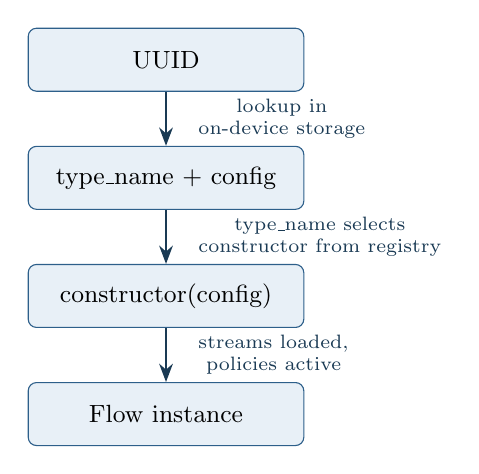
\begin{tikzpicture}[
  box/.style={draw=rimblue, fill=rimlight, rounded corners=3pt, minimum width=3.5cm,
              minimum height=0.8cm, font=\small, align=center},
  arr/.style={->, >=Stealth, thick, color=rimdark},
  label/.style={font=\scriptsize\color{gray}, align=center},
]
  \node[box] (uuid) at (0, 0) {UUID};
  \node[box] (config) at (0, -1.5) {type\_name + config};
  \node[box] (ctor) at (0, -3) {constructor(config)};
  \node[box] (flow) at (0, -4.5) {Flow instance};

  \draw[arr] (uuid) -- (config) node[midway, right=8pt, label] {lookup in\\on-device storage};
  \draw[arr] (config) -- (ctor) node[midway, right=8pt, label] {type\_name selects\\constructor from registry};
  \draw[arr] (ctor) -- (flow) node[midway, right=8pt, label] {streams loaded,\\policies active};
\end{tikzpicture}
\end{center}

A new device joining a flow needs only the configuration. It does not even need the type
map if it can assume the type is correct (because flows are defined at the application
level---the app already knows what type it expects).

From the application's perspective, the entire bootstrap is:
\begin{pseudocode}[Application Bootstrap]
\begin{verbatim}
let flow = registry.load(uuid, &storage)?;
let state = flow.stream("current_state")?.read()?;
// done. UI populates, edits work.
\end{verbatim}
\end{pseudocode}


% ============================================================
\newpage
\section{Streams}
\label{sec:streams}

Streams are the basic I/O primitive of flows. A flow contains streams. Applications
read from and write to streams. Everything that enters or leaves a flow goes through
a stream.

\subsection{What a Stream Is}

A stream is a named, typed channel within a flow through which serialized data moves.
Streams have:

\begin{itemize}[leftmargin=2em]
  \item A \textbf{name}, unique within the flow, given in the schema
  \item A \textbf{cardinality}: singleton (one per flow), per-party (one per participant),
    or unbounded (created as needed, e.g., threads or topics)
  \item A \textbf{category hint}: drip, jet, or unspecified
  \item An \textbf{interface}: read, write, subscribe
\end{itemize}

The category hint is a shorthand for the stream's behavioral contract, not a type
enforced by the system. ``Drip'' and ``jet'' do not appear in function signatures.
They appear in flow type definitions as familiar labels that let readers skip past
long formal names.

\subsection{Drips: Convergent Streams}

\begin{definition}[Drip]
A drip is a stream that provides eventually consistent, authoritative data. Any holder
of a drip should give the same answer after a settling time. Drips are slow, deliberate,
and represent consensus.
\end{definition}

Drips are typically backed by some form of convergent data structure (CRDT, operational
transform, or similar). The backing implementation is injected by the parties responsible
for the drip, not specified by the stream abstraction itself.

Examples of drips:
\begin{itemize}[leftmargin=2em]
  \item The current merged state of a task graph (Giantt)
  \item The current structure of a photo album (order, crops, annotations)
  \item The current consensus alignment of a coordinate system network (Nestbox)
  \item The current merged state of a personal inventory
\end{itemize}

\subsection{Jets: Fast Streams}

\begin{definition}[Jet]
A jet is a stream that provides fast, possibly lossy, real-time data. Jets prioritize
promptness over completeness or consensus.
\end{definition}

Jets carry live interaction data: cursor positions, typing indicators, sensor readings,
video frames, audio samples. Data on a jet may arrive out of order, may be incomplete,
and is not expected to be the same from every observer's perspective.

Examples of jets:
\begin{itemize}[leftmargin=2em]
  \item Who is currently viewing or editing what in a shared photo album
  \item Live audio streams during a group call
  \item Real-time motor encoder readings from a robot arm
  \item IMU and camera data from a phone participating in spatial alignment
\end{itemize}

\subsection{Stream Lifecycle}

Streams defined in the schema exist conceptually from the moment the flow is created.
Whether data is returned from a stream depends on whether any party has implemented it.
If no party is serving a stream, requests to it activate the flow's error policy (which
might return ``data not available,'' retry, fall back to another party, etc.).

New streams can be created according to the schema's rules (e.g., a per-party stream
is created when a new party joins). Streams are not deleted, but may become inactive
if all parties stop serving them. The flow's policies determine what happens when
inactive streams are queried.


% ============================================================
\newpage
\section{Data Geometry}
\label{sec:geometry}

Different kinds of data have fundamentally different spatial, temporal, and structural
character. A protocol that aims to handle images, sound, 3D measurements, task graphs,
and binary blobs through the same flow abstraction must have a way to describe these
differences so that operations like \emph{query}, \emph{subset}, \emph{transform}, and
\emph{merge} can be defined uniformly.

This section defines the vocabulary for describing data geometry. These concepts appear
in flow type definitions and determine what operations streams support.

\subsection{Query Coordinates}

Query coordinates are the dimensions along which you \emph{request} data from a stream.
They define the ``address space'' of the data.

\begin{center}
\begin{tabularx}{\textwidth}{l l l X}
\toprule
\textbf{Data type} & \textbf{Query coords} & \textbf{Type} & \textbf{Notes} \\
\midrule
Binary blob & offset & discrete (integer) & One coordinate. All-or-nothing also valid. \\
Sound & time & continuous (float) & One coordinate. Subsetting = time range. \\
Image & x, y (or u, v) & discrete or continuous & Two ordered coordinates. \\
Video & x, y, time & mixed & Spatial discrete, temporal continuous. \\
3D measurements & x, y, z & continuous & Transforms apply. May include time. \\
Text & line, offset & discrete (integer) & Two coordinates, both ordered. \\
Task graph & item ID & discrete (unordered) & One coordinate, a set of IDs. \\
Inventory & item ID & discrete (unordered) & One coordinate, a set of IDs. \\
Photo album & position & discrete (ordered) & One coordinate: slot in order. \\
\bottomrule
\end{tabularx}
\end{center}

\subsubsection{Properties of Query Coordinates}

Each query coordinate has properties that determine what operations are meaningful:

\begin{itemize}[leftmargin=2em]
  \item \textbf{Discrete vs.\ continuous}: Can you request data at integer indices only
    (pixels, bytes, lines), or at arbitrary real-valued positions (time in seconds,
    spatial position in meters)?
  \item \textbf{Ordered vs.\ unordered}: Does the coordinate have a natural ordering
    (time, position, line number) or is it a set of identifiers (item IDs, UUIDs)?
    Ordered coordinates support range queries; unordered coordinates support set
    membership queries.
  \item \textbf{Bounded vs.\ unbounded}: Is there a known extent (image width, file
    length) or can the coordinate space grow indefinitely (append-only log, growing
    inventory)?
  \item \textbf{Homogeneous vs.\ inhomogeneous}: Are the coordinates in a projective
    space (camera image coordinates often are) where scaling matters, or in an affine
    space where it does not?
\end{itemize}

\subsection{Data Coordinates}

Data coordinates are the dimensions of the \emph{values} returned at each query point.

\begin{center}
\begin{tabularx}{\textwidth}{l l l X}
\toprule
\textbf{Data type} & \textbf{Data coords} & \textbf{Count} & \textbf{Notes} \\
\midrule
Binary blob & byte value & 1 & Technically a bit, practically a byte. \\
Grayscale image & intensity & 1 & \\
RGB image & R, G, B & 3 & \\
RGBA image & R, G, B, A & 4 & \\
Multispectral image & wavelength bands & $n$ & JWST: 29 bands. \\
Sound (mono) & amplitude & 1 & \\
Sound (stereo) & L, R amplitude & 2 & \\
Sound (surround) & channel amplitudes & $n$ & 5.1, 7.1, Atmos, etc. \\
3D position & x, y, z & 3 & Often with covariance. \\
6D pose & x, y, z, roll, pitch, yaw & 6 & Or quaternion: 7. \\
Text & character & 1 & Unicode codepoint. \\
Task graph item & structured record & varies & Title, status, priority, \ldots \\
\bottomrule
\end{tabularx}
\end{center}

\subsubsection{Properties of Data Coordinates}

\begin{itemize}[leftmargin=2em]
  \item \textbf{Discrete vs.\ continuous}: Byte values are discrete (0--255); spatial
    positions are continuous (floats).
  \item \textbf{Scalar vs.\ structured}: A pixel's RGB is a flat vector; a task graph
    item is a structured record with named fields of different types.
  \item \textbf{Uncertain vs.\ exact}: Spatial measurements carry covariance matrices
    quantifying uncertainty. Pixel values are exact (within quantization).
\end{itemize}

\subsection{Transforms}

When query coordinates live in a geometric space (2D, 3D, projective), data can be
requested through a transform. An image flow could accept a $2 \times 2$ matrix and
start/end vectors, returning any rotation, scale, flip, and crop of the image. A 3D
measurement flow could accept a rigid-body transform to return data in a different
coordinate system.

Transforms are part of the query interface, not the data itself. They allow the same
underlying data to be accessed from different perspectives without redundant storage.

\begin{designnote}[Design Decision: Server-side vs.\ Client-side Transforms]
For most data (images at typical resolutions, short audio clips), transforms are better
applied on the receiving device. For very large data (gigapixel images, long high-rate
sensor logs), supporting transforms in the query---so that only the relevant subset
is transmitted---is important. Flow type definitions should specify which transforms
the stream supports in queries.
\end{designnote}

\subsection{Sparsity and Density}

Some data fills its coordinate space densely (images: every pixel has a value). Other
data is sparse (3D feature measurements: values exist at a few scattered points in a
continuous space). The distinction matters for how data is stored, transmitted, and
merged:

\begin{itemize}[leftmargin=2em]
  \item Dense data benefits from array-based storage and compression.
  \item Sparse data benefits from indexed storage (coordinate $\to$ value maps).
  \item Merging two sparse datasets is a set union with conflict resolution at
    coincident points.
  \item Merging two dense datasets requires per-element conflict resolution or
    layer-based composition.
\end{itemize}


% ============================================================
\newpage
\section{Flow Roles}
\label{sec:roles}

\subsection{What a Flow Role Is}

A \emph{flow role} is an abstract unit of responsibility within a flow. Flow roles are
defined in the flow's type definition. Parties (devices, processes, services) \emph{fill}
roles at runtime.

\begin{definition}[Flow Role]
A flow role is a named set of responsibilities defined by a flow type. A single device
can fill many roles. Many devices can fill the same role. Roles are abstract; they do not
imply separate hardware, separate processes, or even separate lines of code---though
they might be any of those.
\end{definition}

The key insight is that hundreds of roles might be filled by a single device, even for
a single flow. A phone running an inventory app might simultaneously fill the roles of
data source (user makes edits), memorization (stores edit history to local files),
fitting (applies edits to produce current state), and data sink (displays current
state in UI). These are all conceptually separate responsibilities that happen to be
co-located.

\subsection{Common Flow Role Types}

\subsubsection{Data Source}

A data source produces new data and writes it to a stream. Examples:
\begin{itemize}[leftmargin=2em]
  \item A user making edits in an app UI
  \item An LLM generating tool calls
  \item A sensor producing readings
  \item A CLI command modifying a task graph
\end{itemize}

\subsubsection{Data Sink}

A data sink consumes data from a stream. Examples:
\begin{itemize}[leftmargin=2em]
  \item A UI displaying the current state of an inventory
  \item A robot arm consuming joint-angle commands
  \item A speaker playing back mixed audio
\end{itemize}

\subsubsection{Memorization}

A memorization flow role reliably stores and recalls data that was written to streams, so
that it can be retrieved later. This is often implemented as local file I/O, but the
flow only specifies the \emph{what} (this data must be recallable under these
conditions) and the \emph{policy} (how robust, how secure, how long), not the
\emph{how}.

Memorization roles carry security policies:
\begin{itemize}[leftmargin=2em]
  \item \textbf{Plaintext-safe}: The host is behind user accounts, passwords, and
    standard security. Data can be stored in plaintext on local drives.
  \item \textbf{Encrypted-at-rest}: The storage location is accessible to others.
    Data must be encrypted before writing.
  \item \textbf{Dissolution-required}: After a time horizon, an attacker would need
    to physically acquire a threshold number of devices to read the data. This triggers
    data dissolution (erasure coding across multiple devices).
\end{itemize}

Memorization roles also carry \textbf{robustness policies}:
\begin{itemize}[leftmargin=2em]
  \item \textbf{Ephemeral}: If the holder disappears, the data is gone. Acceptable for
    transient caches and live-only jets.
  \item \textbf{Replicated}: Data is held by multiple memorization roles. If some
    disappear, others still have it.
  \item \textbf{Reallocating}: If holders disappear over time, the remaining holders
    proactively redistribute data to new roles with updated routes. This is the common
    policy for persistent self-data.
\end{itemize}

\subsubsection{Curator}

A curator grooms raw data for consumption. In the spatial measurement context
(Section~\ref{sec:ex-spatial}), curators remove erroneous measurements, denoise,
and produce summarized measurement sets that aligners query to catch up. Curators
are often co-located with the devices that produce the raw data, but this is a
convenience, not a requirement.

\subsubsection{Aligner}

An aligner is a specialized role for spatial flows (Section~\ref{sec:ex-spatial}).
Aligners consume curated measurements and produce a consensus alignment (a drip)
of coordinate systems. Multiple aligners processing the same data should converge
to the same answer.

\subsection{Fittings}
\label{sec:fittings}

\begin{definition}[Fitting]
A fitting is a transformation that connects streams to each other within a flow.
Fittings describe how data from one stream is processed and made available on another.
\end{definition}

A fitting's functionality is real and implemented in real code---the parties running the
code \emph{are} implementing the fittings described in the flow's policies. But a fitting
is not a first-class named entity at the same level as a stream. There is no fitting
registry, no fitting UUID, no fitting interface that you call methods on. The fitting
is implicit in its implementation: the code that reads from an edit stream, applies
operations to a CRDT, and makes the result available on a drip stream \emph{is} a fitting,
but it does not need to know that about itself.

A fitting might be as simple as ``apply each edit operation from the edit stream to a
CRDT, making the result available on the drip stream,'' or as complex as ``mix $n$ audio
input streams into a single output stream, applying gain normalization and latency
compensation.'' In both cases, the fitting is a description of what the code does, not a
separate object the code instantiates. Delegation policies (\S\ref{sec:policies})
determine which party runs the code that implements a given fitting, and failover
policies determine what happens when that party disappears---but the fitting itself
remains a noun for talking about transformations, not a type for instantiating them.

\begin{center}
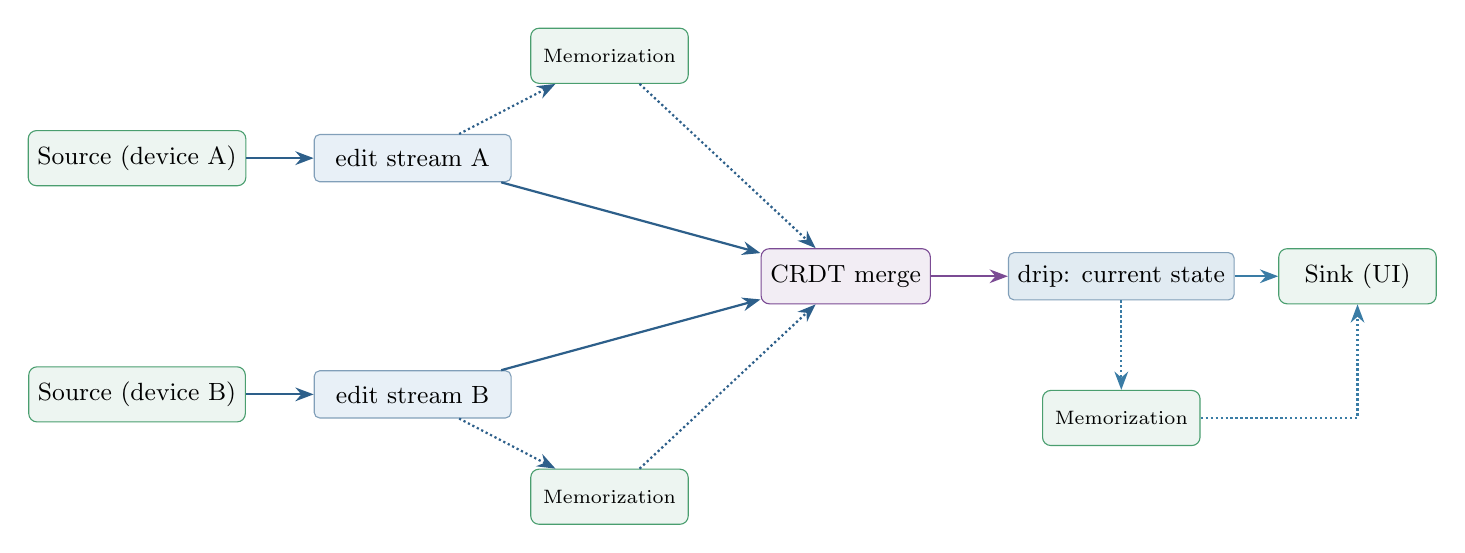
\begin{tikzpicture}[
  stream/.style={draw=rimblue, thick, ->, >=Stealth},
  optional/.style={draw=rimblue, thick, ->, >=Stealth, densely dotted},
  fitting/.style={draw=fittingcolor, fill=fittingcolor!10, rounded corners=3pt,
                  minimum width=2cm, minimum height=0.7cm, font=\small},
  role/.style={draw=rolecolor, fill=rolecolor!10, rounded corners=3pt,
               minimum width=2cm, minimum height=0.7cm, font=\small},
  streambox/.style={draw=rimblue!60, fill=rimlight, rounded corners=2pt,
                    minimum width=2.5cm, minimum height=0.6cm, font=\small},
]
  % Sources
  \node[role] (srcA) at (-5, 1.5) {Source (device A)};
  \node[role] (srcB) at (-5, -1.5) {Source (device B)};

  % Edit streams
  \node[streambox] (editA) at (-1.5, 1.5) {edit stream A};
  \node[streambox] (editB) at (-1.5, -1.5) {edit stream B};

  % Memorization (one per edit stream, forming triangles)
  \node[role] (memA) at (1, 2.8) {\scriptsize Memorization};
  \node[role] (memB) at (1, -2.8) {\scriptsize Memorization};

  % Fitting
  \node[fitting] (fit) at (4, 0) {CRDT merge};

  % Drip
  \node[streambox, fill=dripcolor!15] (drip) at (7.5, 0) {drip: current state};

  % Memorization (read-side, optional, between drip and sink)
  \node[role] (memRead) at (7.5, -1.8) {\scriptsize Memorization};

  % Sink
  \node[role] (sink) at (10.5, 0) {Sink (UI)};

  % Source -> edit stream arrows
  \draw[stream] (srcA) -- (editA);
  \draw[stream] (srcB) -- (editB);

  % Edit streams -> merge directly
  \draw[stream] (editA) -- (fit);
  \draw[stream] (editB) -- (fit);

  % Edit stream A -> memorization A -> merge (triangle)
  \draw[optional] (editA) -- (memA);
  \draw[optional] (memA) -- (fit);

  % Edit stream B -> memorization B -> merge (triangle)
  \draw[optional] (editB) -- (memB);
  \draw[optional] (memB) -- (fit);

  % Merge -> drip
  \draw[stream, color=fittingcolor] (fit) -- (drip);

  % Drip -> sink (direct)
  \draw[stream, color=dripcolor] (drip) -- (sink);

  % Drip -> memorization -> sink (optional detour)
  \draw[optional, color=dripcolor] (drip) -- (memRead);
  \draw[optional, color=dripcolor] (memRead) -| (sink);
\end{tikzpicture}
\end{center}


% ============================================================
\newpage
\section{Policies}
\label{sec:policies}

Policies are the rules encoded in a flow's type definition and configuration that
govern how streams behave under various conditions. They are the ``law'' of the flow:
once you have a flow, the policies call the shots.

\subsection{Error Policies}

What happens when a stream is queried but no party is implementing it? What happens
when a memorization role can't recall data? What happens when a fitting fails?

Error policies specify:
\begin{itemize}[leftmargin=2em]
  \item What abstract error to emit (``data not available,'' ``uninitialized,''
    ``degraded'')
  \item Whether to retry, and how
  \item Whether to fall back to alternative parties
  \item Whether to notify the application or handle silently
\end{itemize}

\subsection{Delegation Policies}

Who performs transmissions and transformations? Delegation policies specify:
\begin{itemize}[leftmargin=2em]
  \item Which roles are responsible for which streams
  \item Whether responsibility can be transferred
  \item How new parties are assigned roles when they join
  \item How roles are redistributed when parties leave
\end{itemize}

\subsection{Discovery Policies}

How do pieces in a capsule find each other when they need to form an ensemble?
Discovery policies specify:
\begin{itemize}[leftmargin=2em]
  \item \textbf{Proximity broadcast}: Pieces advertise presence and capsule membership
    via encrypted BLE advertisements. Other pieces holding the capsule's key material
    can detect and respond. This is the baseline discovery mechanism.
  \item \textbf{Simple}: The flow configuration contains a static list of known pieces
  \item \textbf{Referral}: A known piece can provide the identities of others
  \item \textbf{Registry}: A remote directory service maintains a list of pieces
    (an IP-based extension for when proximity alone is insufficient)
  \item \textbf{DHT}: Distributed hash table lookup (another IP-based extension)
\end{itemize}

The policy also specifies what to do when discovery information is stale (retire the
flow? attempt re-discovery? fall back to a different method?). Because the baseline
is proximity broadcast, staleness often resolves itself: a piece that walks back into
range is rediscovered automatically.

\subsection{Memorization Policies}

How is data stored at rest? Memorization policies combine security and robustness:

\begin{center}
\begin{tabularx}{\textwidth}{l X}
\toprule
\textbf{Policy aspect} & \textbf{Options} \\
\midrule
Security at rest & Plaintext-safe, encrypted-at-rest, dissolution-required \\
Robustness & Ephemeral, replicated, reallocating \\
Retention & Indefinite, time-bounded, size-bounded, policy-on-overflow \\
Provenance & Track origin device and timestamp, or not \\
\bottomrule
\end{tabularx}
\end{center}

\subsection{Retirement and Refresh}

Flows are persistent by nature, but they can be retired. Retirement means no new data
is accepted on any stream, and existing data is subject to the memorization retention
policy. Some flows benefit from being short-lived and easily refreshed (a quick spatial
alignment session among 3 devices), while others are meant to last indefinitely (a
personal photo album).

The flow's type definition specifies whether retirement is manual, automatic
(time-based, inactivity-based), or not supported.


% ============================================================
\newpage
\section{Data Type Examples}
\label{sec:examples}

This section walks through how diverse types of data map onto the self-data flow
abstraction. Each example defines the data geometry, the streams, the roles, and the
key policies.

The examples are ordered from spatially rich to structurally rich, beginning with data
types that have strong geometric character and progressing toward data types whose
structure is more about relationships and records than about coordinates.

% -----------------------------------------------------------
\subsection{Images}
\label{sec:ex-images}

An image has rich spatial structure. Rather than treating images as a single monolithic
flow, the protocol decomposes image handling into three tiers of flows reflecting a key
insight: raw image data, collaborative composition, and collection management have
fundamentally different data characters and independent lifecycles. A photograph someone
took and stores on their devices does not need multi-party consensus---it is spatial data
you query at a resolution. A collaboratively edited composite (layers, transforms,
annotations) does need consensus on the sequence of edits. A collection of composites
(an album) needs consensus on membership and ordering. These are separate flows, linked
by UUID references in a flow mesh (\S\ref{sec:boundaries}).

\subsubsection{Data Geometry (Base Image)}
\begin{itemize}[leftmargin=2em]
  \item \textbf{Query coordinates}: 2. Either discrete $(x, y)$ as integer pixel
    indices, or continuous $(u, v)$ as floats in $[0, 1]$.
  \item \textbf{Data coordinates}: 3 for RGB, 4 for RGBA, 1 for grayscale, $n$ for
    multispectral (up to 29 for some JWST images).
  \item \textbf{Ordered}: Yes, both query coordinates are ordered.
  \item \textbf{Dense}: Yes, every query point has a value.
  \item \textbf{Transform support}: The full query interface supports a $2 \times 2$
    matrix and a pair of start/end vectors, expressing any rotation, scale, flip, and
    crop. Most transforms are better done on the receiving device, but for very large
    images, the query should support spatial subsetting. A valid starting implementation
    may use discrete resolution tiers (thumbnail, preview, large, full) as the query
    parameter, deferring continuous transform support to later iterations.
\end{itemize}

\subsubsection{Three-Tier Decomposition}

\begin{enumerate}[leftmargin=2em]
  \item \textbf{Image flow} (query-response, neither jet nor drip). Stores raw image
    data and serves it at a requested resolution. Memorization-backed, spatially aware.
    Multiple pieces can memorize the same image; synchronization is ``do you have this
    data?'' not ``what is the consensus state?'' There is no drip because there is no
    multi-party state to converge---the image simply exists as spatial data.

  \item \textbf{Image composite flow} (has a \textbf{drip}). Produces a rendered result
    from one or more image sources plus transforms, overlays, and annotations. The drip
    converges when multiple parties contribute edits---crops, rotations, layer operations,
    filter applications. A simple composite might contain only a genesis operation (``load
    from image flow $X$ at resolution $Y$''); a rich composite might contain dozens of
    layer operations. The composite flow also returns non-image data (vector annotations,
    text overlays) alongside the rendered pixels.

  \item \textbf{Album flow} (has a \textbf{drip}). A convergent collection of composite
    references. Each entry references a composite flow by UUID. The album's edits are
    structural: add, remove, reorder entries, set captions and tags. Image transforms
    (crop, rotate, filter) belong to the composite layer, not the album. See
    \S\ref{sec:ex-albums}.
\end{enumerate}

\subsubsection{Image Flow Streams}
\begin{itemize}[leftmargin=2em]
  \item \textbf{Image data} (query-response, no category): Returns image data at a
    requested resolution. The resolution parameter is part of the query. This is neither
    a drip (no multi-party consensus to fuse) nor a jet (not continuous or lossy).
  \item \textbf{Metadata} (read-once, no category): Dimensions, format, original size,
    color space.
\end{itemize}

\subsubsection{Image Composite Flow Streams}
\begin{itemize}[leftmargin=2em]
  \item \textbf{Drip} (\texttt{operations}): The convergent sequence of composition
    operations. When multiple parties contribute edits (transforms, layers, annotations),
    the drip ensures convergence via its backing CRDT.
  \item \textbf{Rendered} (query-response, no category): The composited image data plus
    extra data (annotations, vectors) at a requested resolution.
  \item \textbf{Jet} (\texttt{viewport}): Per-party, what region of the composite each
    participant is currently viewing. Optional; useful for collaborative editing UIs.
\end{itemize}

\subsubsection{Key Policies}
\begin{itemize}[leftmargin=2em]
  \item Conflict resolution for concurrent composition edits: operation ordering via the
    drip's backing CRDT.
  \item Large images: memorization roles may store tiles or resolution tiers, serving
    subsets on query.
  \item The image flow and the composite flow referencing it have independent lifecycles:
    the same raw image can appear in many composites; retiring a composite does not affect
    the underlying image data.
\end{itemize}

% -----------------------------------------------------------
\subsection{Video}
\label{sec:ex-video}

Video extends images with a time coordinate.

\subsubsection{Data Geometry}
\begin{itemize}[leftmargin=2em]
  \item \textbf{Query coordinates}: 3. Spatial $(x, y)$ plus temporal $t$ (continuous).
  \item \textbf{Data coordinates}: Same as image (RGB, RGBA, etc.).
  \item \textbf{Dense in space, dense or sparse in time}: Every pixel in a frame has
    a value; frames may be keyframes with interpolation between them.
\end{itemize}

\subsubsection{Streams}
\begin{itemize}[leftmargin=2em]
  \item \textbf{Drip} (\texttt{frame\_state}): The consensus sequence of frames.
    Queryable by time range and spatial region.
  \item \textbf{Jets} (per-party): Live camera feeds or screen shares. Fast, lossy,
    per-observer.
  \item \textbf{Edit streams}: Cuts, splices, overlays, filters, applied to the
    temporal structure.
\end{itemize}

\subsubsection{Relationship to Calls and Recordings}

A video call is a self-data flow where each participant contributes a jet (their live
camera feed). Each participant's local recording of the call is itself a data entity:
the truth of what happened at one end, saved locally for reference by other flows
(personal albums, file systems). The flow's drip---the consensus ``what happened''---is
not the same as any participant's live observations. It is the multi-screen,
high-quality reconstruction assembled from all participants' locally stored data, whether
as pointers into their local storage or as a literal instantiated file.

% -----------------------------------------------------------
\subsection{Sound}
\label{sec:ex-sound}

Sound has minimal spatial structure but strong temporal structure and strict latency
requirements during playback.

\subsubsection{Data Geometry}
\begin{itemize}[leftmargin=2em]
  \item \textbf{Query coordinates}: 1. Time $t$ (continuous). Subsetting = time range.
  \item \textbf{Data coordinates}: $n$ channels. Mono: 1. Stereo: 2. Surround: 5.1,
    7.1, Atmos, etc.
  \item \textbf{Free parameters}: Gain, sampling frequency.
  \item \textbf{Ordered, dense in time} (at the sampling rate).
\end{itemize}

\subsubsection{Streams}
\begin{itemize}[leftmargin=2em]
  \item \textbf{Drip} (\texttt{mixed\_audio}): The consensus of what tracks should have
    been playing what when. Equivalent to a full multitrack project (Audacity-like).
  \item \textbf{Jets} (per-party): Live audio input. For a group call, these are the
    participants' microphone streams.
  \item \textbf{Edit streams}: Import clips, manipulate clips (trim, move, gain adjust),
    add/remove tracks. The drip reflects the consensus edit state; querying it causes
    mixing to happen at the specified sampling frequency.
\end{itemize}

\subsubsection{Latency and Decompression}

Sound must be incredibly prompt during playback. It is better to insert filler
(silence, comfort noise, interpolation) than to break the stream and restart. This
motivates:

\begin{itemize}[leftmargin=2em]
  \item Jets return data in a format designed to be fed into decompression and
    smoothing.
  \item A trivial decompressor (passthrough) is a simple fitting from jet to OS audio
    output.
  \item Smarter decompressors may want richer data (prediction residuals, codebook
    info) from the jet to do more intelligible gap-filling. This is an open design
    question: how much metadata to include in the jet format.
\end{itemize}

\begin{designnote}[Starting Big]
It might be better to start big with sound, just as with text (Section~\ref{sec:ex-text}):
all sounds are playbacks of collections of tracks with clips. A phone call is clips
continuously imported into separate tracks. Querying causes mixing. This avoids
special-casing simple scenarios and immediately generalizes.
\end{designnote}

% -----------------------------------------------------------
\subsection{Spatial Measurements}
\label{sec:ex-spatial}

Spatial measurement flows support the distributed, multi-device, multi-coordinate-system
alignment problem. This is the domain of Nestbox, where devices with different sensors
(cameras, IMUs, LIDAR, robot encoders) observe shared features in a physical space and
must agree on how their coordinate systems relate.

\subsubsection{Data Geometry}
\begin{itemize}[leftmargin=2em]
  \item \textbf{Query coordinates}: 3D (or 6D with velocity, or 2D for some sensors).
    Continuous. Subject to coordinate system transforms.
  \item \textbf{Data coordinates}: Multivariate Gaussian. Mean vector plus precision
    (inverse covariance) matrix. Dimensionality, cardinality, and whether the
    measurement is projective are all flexible.
  \item \textbf{Sparse}: Measurements exist at scattered points, not densely.
  \item \textbf{Uncertain}: Every measurement carries quantified uncertainty.
\end{itemize}

\subsubsection{Why Precision Matrices}

Precision matrices (inverse covariance) should be preferred over covariance matrices
throughout. They save unnecessary inversions (many optimization algorithms work natively
in information form), compose more naturally for independent measurements, and avoid
numerical issues with near-singular covariances.

\subsubsection{Coordinate Systems}

Each device cares about certain coordinate systems. A flow bundles coordinate systems
and defines transforms between them. The transforms are maintained by aligners and
served as drips.

A device that can move but not measure (a basic robot arm) needs only to receive a
transform from a drip to convert commands in one coordinate system to its local frame.

\subsubsection{Streams}

This flow type has an unusually large number of streams:

\begin{itemize}[leftmargin=2em]
  \item \textbf{Drips}:
    \begin{itemize}
      \item Per-aligner: current best-effort alignment (all should converge)
      \item Curated measurements: the denoised, pruned measurement set
    \end{itemize}
  \item \textbf{Jets}: Raw measurements from each device, streamed to aligners/curators
  \item \textbf{Historical streams}: Measurement histories, alignment state histories,
    for new aligners catching up
\end{itemize}

\subsubsection{Flow Roles}
\begin{itemize}[leftmargin=2em]
  \item \textbf{Sensor}: Data source. Produces raw measurements in its local
    coordinate system.
  \item \textbf{Curator}: Grooms measurements. Removes outliers, denoises, summarizes.
    Often co-located with sensors due to data proximity.
  \item \textbf{Aligner}: Consumes curated measurements, produces consensus alignment.
    Multiple aligners should converge.
  \item \textbf{Consumer}: Reads alignment drips to get transforms. May be a robot arm
    that just needs to know how to convert coordinates.
\end{itemize}

\subsubsection{Flow Boundaries}
\label{sec:ex-spatial-boundaries}

Should the alignment session be one big flow or many small ones? Key considerations:

\begin{itemize}[leftmargin=2em]
  \item A ``current effort with the devices that are here now'' should be easy to
    retire or refresh after use.
  \item Long-lived persistent alignment data might live in a different flow.
  \item Many flows can form a mesh---not everyone needs to be on one huge global flow.
  \item A new flow can be announced briefly among, say, 3 devices.
\end{itemize}

See Section~\ref{sec:boundaries} for general principles.

\subsubsection{Relationship to Nestbox Twigs}

The existing Nestbox Twig system (Protocol Buffers, \texttt{SampleRouter}, dimension
enums) implements exactly the sensor-to-aligner path described above, but with bespoke
plumbing per use case. The Twig's \texttt{stream\_id} and \texttt{coord\_sys\_id} map
to stream identity within a flow. The \texttt{MeasurementSet} with its dimensions,
covariance, transforms, and homogeneity flags maps to the data geometry vocabulary
defined in Section~\ref{sec:geometry}. The \texttt{SampleRouter} is a fitting.

What Twigs lack is the flow-level abstraction: no UUID bundling streams, no policies
for memorization/discovery/error, no schema declaring what streams exist. Every new
device type requires new bespoke routing configuration. Self-data flows generalize
the pattern.

% -----------------------------------------------------------
\subsection{Photo Albums}
\label{sec:ex-albums}

A photo album is a self-data flow whose data is a convergent collection of references
to image composite flows (\S\ref{sec:ex-images}). Each album entry references a
composite flow by UUID; the album reads from the composite to obtain image data for
display, ignoring the composite's non-image data (annotations, vectors) unless the
UI chooses to present it.

The album's concerns are structural: what composites are in the collection, in what
order, with what captions and tags. Image-level transforms (crop, rotate, filter)
belong to the composite layer---the same image can appear in two albums with different
crops, because the crops are properties of different composite flows, not of the album
entries.

\subsubsection{Streams}
\begin{itemize}[leftmargin=2em]
  \item \textbf{Drip} (\texttt{album\_state}): The current structure of the album.
    Queryable for the ordered list of entries, each entry's composite flow UUID, caption,
    tags, and album-level metadata. Backed by a ConvergentDocument.
  \item \textbf{Edit streams} (per-party): Add entry (referencing a composite flow),
    remove entry, reorder, set caption, add/remove tags. These are purely structural
    operations on the collection; no image data passes through the album's edit streams.
  \item \textbf{Jets} (per-party): Who is currently viewing what, who is typing a
    comment where. Prompt, non-consensus.
\end{itemize}

\subsubsection{Flow Roles}
\begin{itemize}[leftmargin=2em]
  \item Standard: data source (editor), data sink (viewer), memorization (stores album
    state), fitting (applies structural edits to album CRDT).
\end{itemize}

% -----------------------------------------------------------
\subsection{Binary Data}
\label{sec:ex-binary}

A block of binary data is the simplest self-data flow. It has no \emph{a priori}
knowable internal structure; you can only have it all-or-nothing (or by byte offset).

\subsubsection{Data Geometry}
\begin{itemize}[leftmargin=2em]
  \item \textbf{Query coordinates}: 1. Offset from start (discrete, integer).
  \item \textbf{Data coordinates}: 1. Byte value (discrete, 0--255).
  \item \textbf{Ordered, bounded} (known length).
\end{itemize}

\subsubsection{Streams}
\begin{itemize}[leftmargin=2em]
  \item \textbf{Drip}: The most recent version with edits integrated. Conflict
    resolution is crude (e.g., if two parties insert at the same offset, one wins per
    policy---this is explicitly undefined/policy-dependent).
  \item \textbf{Edit streams}: Append, prepend, insert at offset, complete replacement
    (most common).
\end{itemize}

% -----------------------------------------------------------
\subsection{Structured Records: Inventory}
\label{sec:ex-inventory}

A personal inventory is a collection of items with properties. It maps naturally to a
ConvergentDocument-backed drip.

\subsubsection{Data Geometry}
\begin{itemize}[leftmargin=2em]
  \item \textbf{Query coordinates}: 1. Item ID (discrete, unordered set).
  \item \textbf{Data coordinates}: Structured record (name, quantity, location, tags,
    custom fields). Variable per item.
\end{itemize}

\subsubsection{Current Implementation and Migration Path}

The current inventory app uses a Dart CRDT with file-based operation logs. The migration
to a self-data flow means:

\begin{enumerate}[leftmargin=2em]
  \item The flow UUID stands for one complete inventory.
  \item The flow's type determines what modules are loaded for memorization (local
    file I/O for now) and fittings (CRDT apply for the drip).
  \item The app reads from the drip (current inventory state) and writes to an edit
    stream (commands).
  \item Memorization: edit histories are accumulated in per-stream files, as they are
    now. The only change is that the behavior is loaded as a module from the flow,
    so it could be swapped for dissolution, network storage, etc.\ without the app
    knowing.
  \item Other devices' edits arrive as additional streams. Their histories are stored
    the same way. The fitting merges all streams into the drip.
\end{enumerate}

\begin{designnote}[Dart CRDT vs.\ Rust Port]
Two paths for the CRDT implementation:
\begin{enumerate}
  \item Port the Dart CRDT to Rust (like Giantt). Clean, everything in soradyne\_core.
  \item Keep the Dart CRDT; soradyne integration invokes it via callback/binding as
    the fitting implementation for the drip.
\end{enumerate}
The decision depends on whether the Dart CRDT has features that would be expensive to
reimplement, and whether the callback overhead is acceptable. For consistency with
Giantt, porting to Rust is recommended.
\end{designnote}

% -----------------------------------------------------------
\subsection{Task Graphs: Giantt}
\label{sec:ex-giantt}

A Giantt task graph is a collection of items with typed relations (REQUIRES, ANYOF,
BLOCKS, etc.), time constraints, status, priority, and tags. It is a structured record
flow with graph semantics.

\subsubsection{Data Geometry}
\begin{itemize}[leftmargin=2em]
  \item \textbf{Query coordinates}: 1. Item ID (discrete, unordered set). But graph
    structure imposes a partial order via dependencies.
  \item \textbf{Data coordinates}: Structured record (title, status, priority, duration,
    time constraints, tags, charts, relations to other items).
\end{itemize}

\subsubsection{Streams}
\begin{itemize}[leftmargin=2em]
  \item \textbf{Drip} (\texttt{graph\_state}): The current merged task graph. Backed
    by a ConvergentDocument with GianttSchema.
  \item \textbf{Edit streams} (per-party): Add/remove items, set fields, add/remove
    relations. Each edit carries causal context (horizon).
\end{itemize}

\subsubsection{Current Implementation}

The Rust ConvergentDocument with GianttSchema already implements the drip backing.
The Dart CLI and Flutter app produce edits. The migration wraps these in a flow so
that the CRDT, the edit source, and the memorization are all accessed through the flow
by UUID, with the fitting logic loaded from the flow's type.

% -----------------------------------------------------------
\subsection{Text}
\label{sec:ex-text}

Line-based text can be managed by well-understood conflict-resolved diff methods.

\subsubsection{Data Geometry}
\begin{itemize}[leftmargin=2em]
  \item \textbf{Query coordinates}: 2. Line number and character offset (both discrete,
    ordered). Or: 1, just byte offset.
  \item \textbf{Data coordinates}: 1. Character (Unicode codepoint).
\end{itemize}

\subsubsection{Starting Big: File Trees}

The default text flow type should represent an entire file tree: prefixed names mapped
to IDs. A single-file flow contains one name (\texttt{/}) mapped to one ID (hash of
flow ID). Multi-file flows map paths to IDs. All multi-diffs always apply atomically
to all text they regard, like git.

\subsubsection{Streams}
\begin{itemize}[leftmargin=2em]
  \item \textbf{Drip}: Merged text state. Queryable by file path, line range, offset.
  \item \textbf{Edit streams}: Groups of diffs (insertions, deletions, replacements)
    with causal context.
\end{itemize}

\begin{designnote}[Text is De-Emphasized]
Text-based CRDTs are a well-studied problem and an easy one to articulate. The Rim
protocol's text support is important but not foundational. The examples above (images,
sound, spatial measurements) are more representative of the protocol's intended scope
and the kinds of problems it uniquely addresses.
\end{designnote}

% -----------------------------------------------------------
\subsection{Vector Images}
\label{sec:ex-vector}

Vector images are structured text (XML for SVG, AI format, etc.) but are not truly
text---they have symmetries (reordering tags, grouping elements) that line-based diff
does not respect.

\subsubsection{Open Question}

Should vector image flows be built on a structured-text flow that respects XML/HTML/JSON
symmetries (reordering, nesting), with SVG as one application? Or should SVG flows be
derived independently? The structured-text approach is more general but harder. The
direct approach risks reinventing the wheel for each structured format.

Operations that would be faithful to vector image semantics: merge by groups, select
by inclusive/exclusive box bounds, select by group or symbol identity.


% ============================================================
\newpage
\section{The Implementer's Perspective}
\label{sec:implementers}

\subsection{Defining a New Flow Type}

To define a new flow type:

\begin{enumerate}[leftmargin=2em]
  \item Write a design document specifying all streams, roles, policies, data geometry,
    and the application-facing interface.
  \item Serialize the design document to a canonical form and compute its content hash.
    This hash is the type identity.
  \item Tag the hash with a human-readable name and version string for convenience.
  \item Implement the type's constructor, which accepts a \texttt{FlowConfig} and
    returns a \texttt{Flow} with the right streams and policies.
  \item Register the constructor in the \texttt{FlowRegistry} under the type name
    (or hash).
\end{enumerate}

The design document is the source of truth. Implementations in different languages
conform to the design document, not to each other's code. The hash ensures that
everyone agreeing on a type hash is agreeing on exactly the same specification.

\subsection{Cross-Language Implementation}

The Rim protocol is designed to be implemented in multiple languages. The Rust
implementation in \texttt{soradyne\_core} is the reference, but applications in Dart,
Python, C\#, Swift, etc.\ should be able to:

\begin{enumerate}[leftmargin=2em]
  \item Provide a UUID to an interface object (in their language) backed by the
    Rim protocol.
  \item Treat the resulting object as having a known type with a known interface.
  \item Read from streams, write to streams, subscribe to updates.
\end{enumerate}

This works because flow types are defined by design documents (the ``PDF''), not by
Rust structs. An implementer in Python reads the design document and implements the
same streams, roles, and policies. The content hash of the type ensures compatibility
can be verified.

\subsection{Extending vs.\ Replacing}

Many roles defined in flow type design documents are ``drop-in'': generic memorization,
generic discovery, generic error handling. These are provided by the Soradyne
distribution and can be used by any flow type.

Some flow types innovate on specific roles (a novel alignment algorithm, a specialized
compression scheme) while keeping the generic roles for everything else. The plugin
architecture supports this: register a flow type constructor that wires together
standard modules for most roles and custom code for the novel parts.

Flows on minimal hardware (ESP32, embedded Linux) may use stripped-down implementations
of standard roles. The flow type's design document describes the interface; the
implementation is whatever fits on the device.

\subsection{What Ships with Soradyne}

The Soradyne distribution includes:

\begin{itemize}[leftmargin=2em]
  \item Several built-in flow types (inventory, task graph, photo album, binary blob)
  \item Pre-made configurations for each type
  \item UUIDs that index those configurations
  \item A library of standard role implementations (local file memorization,
    in-memory streams, basic discovery, ConvergentDocument for drips)
\end{itemize}

A new device joining an existing flow needs only the configuration. After that, just
UUIDs. ``Load flow X'' $\to$ UI populates, edits work.


% ============================================================
\newpage
\section{Security and Memorization}
\label{sec:security}

\subsection{Data at Rest}

Every memorization role operates under a security policy specified by the flow. The
three tiers:

\begin{enumerate}[leftmargin=2em]
  \item \textbf{Plaintext-safe}: Host is behind standard security (user accounts,
    passwords). Data stored in plaintext.
  \item \textbf{Encrypted-at-rest}: Storage location is accessible to others. Data
    encrypted before writing, keys managed by the flow's authentication system.
  \item \textbf{Dissolution-required}: After a time horizon, an attacker must
    physically acquire a threshold number of devices to read the data. Implemented
    via data dissolution (erasure coding across devices using Reed-Solomon or similar).
\end{enumerate}

\subsection{Data Dissolution and Crystallization}

Data dissolution splits data across multiple devices using erasure coding. No single
device holds enough to reconstruct the data. Crystallization is the reverse: when
enough devices come together, the data can be reconstructed.

The flow's memorization policy specifies:
\begin{itemize}[leftmargin=2em]
  \item The threshold: how many devices are needed to crystallize
  \item The total: how many devices hold shards
  \item The time horizon: after how long dissolution is required
  \item Reallocation: what happens when shard-holding devices disappear
\end{itemize}

\subsection{Robustness to Loss}

The most common robustness policy for persistent self-data is \textbf{reallocating}:
if holders of memorization roles disappear over time, the remaining holders proactively
redistribute data to new roles with updated routes. This ensures that even if every
original host were to disappear a few at a time over a long period, the data survives
by continuously migrating to new hosts.

This is distinct from simple replication. Replication assumes a static set of holders.
Reallocation assumes a dynamic set and actively manages the transitions.

\subsection{Leakage Policies}

Memorization policies must specify the level of leakage allowed: what happens if
someone outside the Rim ecosystem looks at the stored data? This determines whether
plaintext, encryption, or dissolution is required.

\subsection{Authentication and Authorization}

Every exchange of information through a flow confirms identity and authorization.
This is part of the policies for streams and drips:

\begin{itemize}[leftmargin=2em]
  \item Who is authorized to write to each stream
  \item Who is authorized to read from each stream
  \item How authorization is verified (signatures, tokens, challenge-response)
  \item What happens on authorization failure
\end{itemize}


% ============================================================
\newpage
\section{Flow Boundaries}
\label{sec:boundaries}

When should something be one flow vs.\ multiple flows? The guiding principle:

\begin{definition}[Flow Boundary Principle]
A self-data flow's boundary is defined by the streams and drips that \emph{must} be
fitted back to each other invisibly from the perspective of users of the Rim protocol
API. If interconnections can be managed by splitting into several flows, each managed
independently by an application, and information shuttled between them in ways the
application would naturally expect, then they should be separate flows.
\end{definition}

\textbf{Example}: ``Get a photo'' should involve only one flow, even if Soradyne
engages many devices in multiple steps to fetch it. ``Move a photo to a new album
that you got from an older one'' naturally involves two flows at the application level.

\subsection{Guidelines}

\begin{itemize}[leftmargin=2em]
  \item \textbf{Atomic unit of data}: If the data makes no sense without all its parts
    (an image's pixels, an inventory's items), it's one flow.
  \item \textbf{Independent lifecycle}: If parts of the data should be retirable
    independently (a temporary spatial alignment session vs.\ persistent calibration
    data), they should be separate flows.
  \item \textbf{Participant scope}: If not all participants need all data, separate
    flows avoid forcing everyone onto one big global flow. A mesh of many small flows
    is often better.
  \item \textbf{Application-natural boundaries}: If the application would naturally
    treat something as two separate entities (two albums, two inventories, two task
    lists), they should be separate flows.
\end{itemize}

\subsection{Flow Mesh}

Multiple flows can reference each other. A photo album flow contains references (by
UUID or content hash) to image data that may live in separate binary-blob flows or
image flows. This creates a mesh of flows, each independently managed, discoverable,
and retirable, but linked by references.

The mesh is not a protocol-level construct---it emerges from applications storing
references to other flows' UUIDs in their data. But the protocol should make this
easy by ensuring that UUIDs are stable, discoverable, and sufficient to bootstrap
access.


% ============================================================
\newpage
\section{Device Topology: Capsules, Ensembles, and Pieces}
\label{sec:topology}

Previous sections describe flows, streams, roles, and policies in terms of abstract
\emph{parties}---anything that can fill a role. This section specifies how devices are
grouped, authorized, and tracked at the physical and network level. The terminology is
drawn from fashion and jewelry, where items are curated into coordinated sets, worn in
varying combinations, and sometimes sold as matched collections.

\subsection{Cryptographic Identity as Foundation}

Everything in the device topology---capsule membership, encrypted advertisements,
pairing verification, flow authentication---depends on cryptographic device identity.
This is not a feature that can be added later; it is the non-negotiable foundation that
all other layers build on.

Each piece has an Ed25519 signing keypair (for authentication and signing operations)
and an X25519 key-agreement keypair (for establishing shared secrets during pairing
and encrypting communications). Together these form the cryptographic root of a piece's
identity. The signing key proves ``I am who I claim to be''; the key-agreement key
enables ``we can talk privately.''

When a capsule is created, shared symmetric key material is established and distributed
to all members during the pairing step. This key material enables encrypted BLE
advertisements (so only capsule members can detect each other) and per-session encryption
of data connections. Key material is bound to the capsule, not to individual connections.

These primitives---per-device identity keypairs and per-capsule shared keys---are the
minimum viable cryptographic infrastructure. They must exist before any capsule can be
built, any ensemble can form, or any flow can authenticate its participants. The
protocol treats their implementation as a prerequisite, not an extension.

\subsection{Pieces}

A \textbf{piece} is a device considered as a member of one or more device groupings. The
word is deliberately neutral: a phone is a piece, a laptop is a piece, an ESP32 is a
piece, a robot arm is a piece. What makes something a piece (rather than just ``a
device'') is that it participates in the Rim protocol's device topology---it has been
authorized into at least one capsule.

A piece can belong to many capsules simultaneously. Its identity within the protocol is
tied to its cryptographic device identity, not to any particular capsule membership.

\subsection{Capsules}

A \textbf{capsule} is a persistent, curated set of pieces that have been authorized to
work together. The term is used in the fashion sense: a capsule wardrobe is a set of
items designed or curated so they can all work together and mix-and-match. A device
capsule is a set of devices authorized to see each other, coordinate, and route traffic
among themselves when they happen to be nearby.

Capsules have the following properties:

\begin{itemize}[leftmargin=2em]
  \item \textbf{Built incrementally}: Pieces are authorized into a capsule one or a few
    at a time, using trustworthy out-of-band linking strategies (QR codes, NFC tap,
    proximity-based challenge-response, or similar). The authorization step establishes
    mutual trust between the new piece and the existing capsule membership.
  \item \textbf{Relatively persistent}: A capsule is meant to be a stable, long-lived
    grouping. You build it over time as you acquire or designate devices for a purpose.
  \item \textbf{Retired whole}: In the style of proactive security, the preferred
    response to a compromised or lost piece is to retire the entire capsule and build a
    new one, re-authorizing each remaining piece. This is analogous to key rotation: you
    do not subtract from a capsule, you replace it. Subtraction would leave ambiguity
    about what the removed piece still knows or can do.
  \item \textbf{Multi-membership}: A piece can belong to many capsules. A phone might be
    in a ``daily carry'' capsule with a watch and earbuds, a ``home studio'' capsule with
    a laptop and audio interface, and a ``lab'' capsule with a set of sensors.
\end{itemize}

\subsubsection{Capsules as Pre-Flow Infrastructure}

Capsules are not flows. They are infrastructure that flows depend on. A flow needs a
capsule to know who the participants are, what keys to use for encrypted communication,
and what the ensemble topology looks like. Making capsules a flow would create a
bootstrapping dependency: you would need a working flow evaluation to load the capsule
that tells you who to sync flows with.

A capsule's piece set is add-only: pieces are authorized in but never individually
removed (the capsule is retired whole instead). This means the merge function is set
union---the simplest possible convergent data structure. Two pieces connect, exchange
their piece sets, take the union, done. No operation logs, no causal tracking, no
conflict resolution beyond deduplication by device identity. This simplicity is
deliberate: it means the same data structure works on a full device and on a
microcontroller with kilobytes of RAM.

\subsection{Ensembles}
\label{subsec:ensembles}

\begin{designnote}[Naming: Ensemble vs.\ Outfit]
The active-subset concept needs a name with the right connotations. Two candidates:

\textbf{Ensemble} is neutral, with a dual meaning as a collection of things considered
as a whole (particularly musicians playing together).

\textbf{Outfit} is construable as a group of people undertaking a particular activity
together, with a secondary fashion meaning.

This document uses \emph{ensemble} as a placeholder. The final choice is pending.
\end{designnote}

An \textbf{ensemble} is the dynamic subset of a capsule's pieces that are currently
online and actively coordinating with each other. Where a capsule is a persistent
authorization list, an ensemble is a live, moment-to-moment reality: who is actually here
right now, responding, and participating in traffic routing.

Ensembles have the following properties:

\begin{itemize}[leftmargin=2em]
  \item \textbf{Real-time membership}: Pieces join and leave ensembles as they come
    online, move into range, or go to sleep. Every participating piece tracks the current
    ensemble membership with both additions and subtractions. A piece is a member of the
    ensemble if it is \emph{reachable}---directly or through intermediaries---not only if
    it has a direct transport-layer connection (see \S\ref{subsec:routing-fabric}).
  \item \textbf{Shared topology picture}: All pieces in an ensemble maintain a shared
    understanding of the current network topology---who is responding, what the
    connectivity graph looks like, and what routes are available. This picture is
    maintained via encrypted advertisements and broadcasts over BLE (or whatever the
    transport layer provides).
  \item \textbf{Associated data structures}: An ensemble may have directed multigraph
    data structures and synchronization states associated with it, representing the live
    routing topology, pending data transfers, and coordination state. These structures
    are maintained collaboratively by all participating pieces.
  \item \textbf{Scoped to a capsule}: An ensemble is always a subset of exactly one
    capsule. A piece that belongs to multiple capsules may participate in multiple
    ensembles simultaneously, but each ensemble draws its membership from a single
    capsule's authorization list.
\end{itemize}

\subsection{Parures}

A \textbf{parure} is a set of pieces that are integrated at the hardware or firmware
level, intended to be together from the beginning. The term comes from jewelry: a parure
is a matched set of pieces (necklace, earrings, bracelet, brooch) designed and sold
together.

In the Rim protocol, a parure is a set of devices that:

\begin{itemize}[leftmargin=2em]
  \item Were sold together, or are part of the same hardware ecosystem
  \item Communicate via specialized, possibly proprietary protocols between themselves
  \item Can be assumed to have solved the internal routing problem---they know how to
    talk to each other efficiently without the general-purpose Rim discovery and topology
    mechanisms
  \item Effectively form a \emph{clique} whenever they appear together in an ensemble:
    every piece in the parure can reach every other piece in the parure directly, with
    known latency and bandwidth characteristics
\end{itemize}

A parure simplifies the ensemble's routing problem. Whenever two or more members of a
parure appear in an ensemble, the topology tracker can treat them as a pre-solved
clique---no discovery or route-finding needed among them---and focus routing decisions
on the links between the parure cluster and the rest of the ensemble.

The near-term hardware development path---starting with individual ESP32-S3
microcontrollers as accessories---is heading toward parures: matched sets of custom
hardware designed and built together, communicating over shared protocols, forming a
pre-solved clique in any ensemble they join.

\subsection{Accessories}

An \textbf{accessory} is a device that can store data or serve some simple, singular role
but is not expected to manage connections in a sophisticated way. Where a full piece runs
the Soradyne/Rim core libraries and participates in ensemble topology tracking and
routing decisions, an accessory implements a minimal interface.

Examples of accessories:
\begin{itemize}[leftmargin=2em]
  \item A microcontroller with storage (e.g., an ESP32 with an SD card) that holds
    dissolution shards
  \item An actuator that receives commands from a flow
  \item A simple bridge to a different device or protocol (e.g., a BLE-to-serial adapter)
\end{itemize}

Most accessories participate in the transport fabric like any other piece---they route
traffic through themselves when they sit between two other pieces in the topology
(see \S\ref{subsec:routing-fabric}). Routing requires only forwarding opaque envelopes
based on destination headers, which is cheap enough for most microcontrollers. A few
genuinely constrained devices (e.g., an actuator with a unidirectional radio, or a
sensor that can only transmit) may lack the capability to route; this is the exception,
not the rule. The key design constraint is that implementing an accessory should be
straightforward: a small interface, minimal dependencies, no requirement for the full
Soradyne library stack. This makes it feasible to build accessories on
resource-constrained hardware.

\subsection{Transport Philosophy}
\label{subsec:transport-philosophy}

\begin{designnote}[Why BLE First]
Most networking protocols treat IP-based transports (TCP sockets, HTTP, WebSockets) as
the baseline and wireless or hardware-specific transports as extensions. Rim inverts
this deliberately.

BLE is the prototypical transport because it embodies the physical reality the protocol
is designed for: devices on or near a person's body, communicating over short distances,
with constrained bandwidth and power budgets, using broadcast-capable radios. The
protocol is locality-centered, body-centered, fashion-centered, and hardware-centered.

A stream's baseline implementation targets BLE or simulated-BLE semantics. Extending or
replacing this with TCP, UDP, or other IP-based transports is possible but represents
\emph{additional} development effort, not the default path. This ensures that the
simplest, most natural deployment---a person's devices talking to each other in
proximity---works without any network infrastructure.
\end{designnote}

Ensemble topology maintenance is expected to rely heavily on BLE's broadcast and
advertising capabilities:

\begin{itemize}[leftmargin=2em]
  \item \textbf{Encrypted advertisements}: Pieces advertise their presence and capsule
    membership via encrypted BLE advertisement packets. Only pieces holding the capsule's
    shared key material can decode these advertisements.
  \item \textbf{Topology synchronization}: When pieces discover each other via
    advertisements, they establish connections and synchronize their view of the ensemble's
    directed multigraph---who can reach whom, through what paths, at what quality.
  \item \textbf{Graceful extension}: An implementation may extend a BLE-based ensemble
    with IP-based links (e.g., when two pieces are on the same WiFi network, or when a
    cloud relay is available). These extensions layer on top of the BLE-first topology,
    they do not replace it.
\end{itemize}

\subsection{Routing as Transport Fabric}
\label{subsec:routing-fabric}

Routing data through intermediate pieces is a \textbf{transport-layer concern}, not a
flow role. Every piece in an ensemble participates in routing: if piece A can reach
piece B, and piece B can reach piece C, then B routes traffic between A and C
transparently. This is analogous to how routers in IP networks forward packets without
knowledge of the application-layer content they carry. A piece functioning as a relay
has no responsibilities regarding the data it shuttles---it need not parse, store, or
understand the flow-level content passing through it.

This is a deliberate architectural separation. Contrast with \emph{memorization}, which
is a flow role (\S\ref{sec:roles}): a memorization role stores data and makes it
retrievable later, which requires understanding the flow's data model (at least enough to
serialize and deserialize). A memorization role's implementation might involve multiple
hops across routing nodes---the point-to-point character of ``store this, recall it
later'' is abstract from the physical path the data takes through the network. The relay
nodes on that path are part of the transport fabric, not participants in the flow.

\subsubsection{Logical Addressing and Message Envelopes}

The mechanism that makes routing invisible to flows is \textbf{logical addressing}.
Messages between pieces are wrapped in envelopes that carry a source identifier, a
destination identifier, and a time-to-live (TTL) counter. An intermediate piece
receiving an envelope checks the destination: if it matches the local piece, the message
is delivered locally; otherwise, the envelope is forwarded to the next hop with a
decremented TTL. The intermediate piece never inspects the payload---it operates
entirely on the envelope headers.

This means a flow sending data to a remote piece uses the same interface regardless of
whether the destination is one hop away or three: \emph{send to this UUID}. The
messaging layer consults the ensemble's directed multigraph to determine the next hop,
handles forwarding through intermediaries, and uses the TTL to break routing loops.
Broadcast messages (destination = all) are forwarded to all neighbors, propagating
through the mesh until TTL is exhausted.

\subsubsection{Reachability vs.\ Direct Connection}

An important consequence of multi-hop routing is that a piece's presence in the ensemble
is determined by \textbf{reachability}, not by having a direct transport-layer connection.
A piece is part of the ensemble if messages can reach it---whether directly (one hop) or
through intermediaries (multiple hops). The ensemble's topology tracks both cases: for
directly connected pieces, the next hop is the piece itself; for indirectly reachable
pieces, the next hop is the neighbor that sits on the path toward them.

This distinction matters because ensembles are often not fully connected. In a
three-piece capsule where the phone and the accessory can each reach the laptop but not
each other, both the phone and the accessory are full ensemble members---the laptop
routes traffic between them. Neither the phone nor the accessory needs to know that
the other is only indirectly reachable; from their perspective, messages simply arrive.

Routing decisions are made by the ensemble's topology manager based on the directed
multigraph of connectivity. The topology manager finds paths, manages retries, and
handles link failures. From the flow's perspective, data written to a stream simply
arrives at its destination; the hops in between are invisible.


% ============================================================
\newpage
\section{Terminology Reference}
\label{sec:terminology}

\begin{center}
\begin{longtable}{l p{10cm}}
\toprule
\textbf{Term} & \textbf{Definition} \\
\midrule
\endhead
\textbf{Self-Data Flow} (or SDFlow) &
  A persistent, typed, UUID-identified bundle of streams with policies for data
  movement, transformation, delegation, and exceptions. The core abstraction of the
  Rim protocol. \\[6pt]

\textbf{Stream} &
  The basic I/O abstraction within a flow. Named, typed, with read/write/subscribe
  interface. All data enters and leaves a flow through streams. \\[6pt]

\textbf{Drip} &
  A stream that provides eventually consistent, authoritative data. Slow, deliberate,
  consensus. Named after the slow, steady nature of a water drip. \\[6pt]

\textbf{Jet} &
  A stream that provides fast, possibly lossy, real-time data. Prompt, per-observer,
  non-consensus. Named after a fast water jet. \\[6pt]

\textbf{Fitting} &
  A transformation connecting streams to each other within a flow. A fitting's
  functionality is real and implemented in real code, but a fitting is not a first-class
  named entity at the same level as a stream---it is implicit in its implementation.
  \\[6pt]

\textbf{Flow Role} &
  A named set of responsibilities within a flow. Filled by parties (devices, processes)
  at runtime. A device can fill many roles; many devices can fill the same role.
  Examples: data source, data sink, memorization, curator, aligner. Often shortened to
  ``role'' in discussion. \\[6pt]

\textbf{Policy} &
  A rule encoded in a flow's type definition or configuration governing stream behavior
  under various conditions: errors, delegation, discovery, memorization, retirement. \\[6pt]

\textbf{Flow Type} &
  A versioned design document specifying a flow's streams, roles, policies, and
  application interface. Identified by the content hash of its canonical serialization.
  Defined at the application level. \\[6pt]

\textbf{Flow Configuration} &
  Instance-specific parameters for a flow: participating parties, network addresses,
  storage quotas, etc. Stored on-device, keyed by flow UUID. \\[6pt]

\textbf{Data Geometry} &
  The description of a data type's spatial, temporal, and structural character: query
  coordinates, data coordinates, their discreteness/continuity/orderedness, and
  supported transforms. \\[6pt]

\textbf{Query Coordinates} &
  The dimensions along which data is requested from a stream. Define the address space.
  \\[6pt]

\textbf{Data Coordinates} &
  The dimensions of values returned at each query point. Define the value space.
  \\[6pt]

\textbf{Memorization} &
  A flow role responsible for reliably storing and recalling stream data. Subject to
  security policies (plaintext, encrypted, dissolved) and robustness policies
  (ephemeral, replicated, reallocating). \\[6pt]

\textbf{Dissolution} &
  Splitting data across multiple devices using erasure coding so that no single device
  holds enough to reconstruct it. \\[6pt]

\textbf{Crystallization} &
  Recombining dissolved data when enough devices come together. \\[6pt]

\textbf{ConvergentDocument} &
  A CRDT engine in soradyne\_core used to implement drip backing stores. Generic over
  a schema that defines item types and fields. \\[6pt]

\textbf{DataChannel} &
  A concrete stream implementation for in-memory pub/sub. Formerly called
  \texttt{SelfDataFlow<T>}. One way to implement a stream, not a flow. \\[6pt]

\textbf{Piece} &
  A device considered as a member of one or more capsules. Any device participating
  in the Rim protocol's device topology. \\[6pt]

\textbf{Capsule} &
  A persistent, curated set of pieces authorized to work together, built incrementally
  via trustworthy linking (QR codes, NFC, etc.). Retired whole rather than shrunk, in the
  style of proactive security. A piece can belong to many capsules. \\[6pt]

\textbf{Ensemble} &
  The dynamic, real-time subset of a capsule's pieces that are currently online and
  coordinating. Membership tracked with additions and subtractions by all participating
  pieces. May have associated directed multigraph data structures. (Name pending; see
  \S\ref{subsec:ensembles} for alternatives.) \\[6pt]

\textbf{Parure} &
  A set of pieces integrated at the hardware or firmware level, intended to be together
  from the start (e.g., sold together, same ecosystem). Form a clique when present in an
  ensemble, with pre-solved internal routing. \\[6pt]

\textbf{Accessory} &
  A device serving a simple, singular role (storage, actuation, bridging) without
  full topology management. Implements a minimal interface; does not require the full
  Soradyne library stack. \\[6pt]

\textbf{Routing} &
  Transport-layer forwarding of data through intermediate pieces. Not a flow role---all
  pieces route transparently, like IP routers, without knowledge of flow-level content.
  Messages are wrapped in envelopes with source, destination, and TTL; intermediate
  pieces forward envelopes without inspecting payloads.
  Distinct from memorization, which is a flow role requiring data-model awareness. \\[6pt]

\bottomrule
\end{longtable}
\end{center}


% ============================================================
\newpage
\section{Appendix: Comparison with Nestbox Twigs}
\label{sec:appendix-twigs}

The Nestbox project's Twig system provides a useful point of comparison, as it
implements a subset of what self-data flows generalize.

\begin{center}
\begin{tabularx}{\textwidth}{l X X}
\toprule
\textbf{Concept} & \textbf{Twig} & \textbf{Self-Data Flow} \\
\midrule
Identity & \texttt{stream\_id} + \texttt{coord\_sys\_id} & Flow UUID \\
Schema & Protobuf message definition & Flow type (design document, content-hashed) \\
Routing & \texttt{SampleRouter} with JSON config & Fittings defined by flow policies \\
Data format & Fixed protobuf (\texttt{MeasurementSet}) & Data geometry described in type \\
Dimensions & Enum (\texttt{X, Y, Z, T, VX, ...}) & Query/data coordinate specification \\
Uncertainty & \texttt{CovarianceMatrix} & Precision matrices (recommended) \\
Transforms & \texttt{TransformationMatrix} per measurement set & Part of query interface \\
Discovery & Bespoke per deployment & Flow discovery policy \\
Memorization & None (live only) & Memorization roles with policies \\
Multi-device & TCP + protobuf, per-connection & Flow bundles all streams, multi-transport \\
\bottomrule
\end{tabularx}
\end{center}

The Twig system does its job well for the specific Nestbox use case. Self-data flows
generalize the pattern so that each new device type or application does not require
new bespoke plumbing.


% ============================================================
\section{Appendix: Status of Current Implementation}
\label{sec:appendix-status}

\begin{center}
\begin{tabularx}{\textwidth}{l l X}
\toprule
\textbf{Component} & \textbf{Status} & \textbf{Notes} \\
\midrule
\texttt{Flow} trait & Implemented & Bootstrap-from-UUID model. Directionally correct. \\
\texttt{FlowRegistry} & Implemented & HashMap-based. Placeholder for on-device storage. \\
\texttt{FlowConfigStorage} & Implemented & In-memory. Needs persistent backend. \\
\texttt{Stream} trait & Implemented & read/write/subscribe interface. \\
\texttt{StreamSpec} & Implemented & drip/jet/singleton/per-party. \\
\texttt{BasicFlow} & Implemented & Schema-validated stream registration. \\
\texttt{DataChannel<T>} & Implemented & Former \texttt{SelfDataFlow<T>}. In-memory pub/sub. \\
\texttt{ConvergentDocument} & Implemented & CRDT engine. Giantt and Inventory schemas. \\
Flow type definitions & Not started & Design documents per this spec. Detailed implementation plan exists (DripHostedFlow, image/composite/album flow types). \\
Real I/O through flows & Not started & Streams are in-memory only. Plan specifies BLE GATT-based sync. \\
Dissolution/crystallization & Partial & Reed-Solomon in storage module, not wired to flows. \\
Nestbox integration & Not started & Twig replacement via spatial measurement flow type. \\
Cryptographic identity & Not started & Plan specifies Ed25519 + X25519 per-device identity, capsule shared keys. Positioned as Phase 0 (prerequisite for all else). \\
Device topology (capsules) & Not started & Plan specifies add-only set with gossip merge. Pre-flow infrastructure (not a CRDT, not a flow). \\
Ensemble tracking & Not started & Plan specifies directed multigraph, encrypted BLE advertisements, topology sync protocol, and a logical messaging layer for multi-hop routing (flows address peers by UUID; routing is invisible). \\
BLE transport & Not started & Plan specifies btleplug (Rust-native) on all hosted platforms, simulated BLE for testing. BLE-first, transport-agnostic to frontends. \\
\bottomrule
\end{tabularx}
\end{center}


\end{document}
